\documentclass{beamer}


\usetheme[secheader]{Boadilla}
\setbeamertemplate{navigation symbols}{}
\usepackage[utf8]{inputenc}
\usepackage[francais]{babel}

\setbeamercolor{alerted text}{fg=blue}

\title{PLATA}

\institute{INRETS}
\author{Florent Kaisser}
\date{28-29 octobre 2010}

\begin{document}






\frame{
	\frametitle{Geographic Information System (GIS)}

  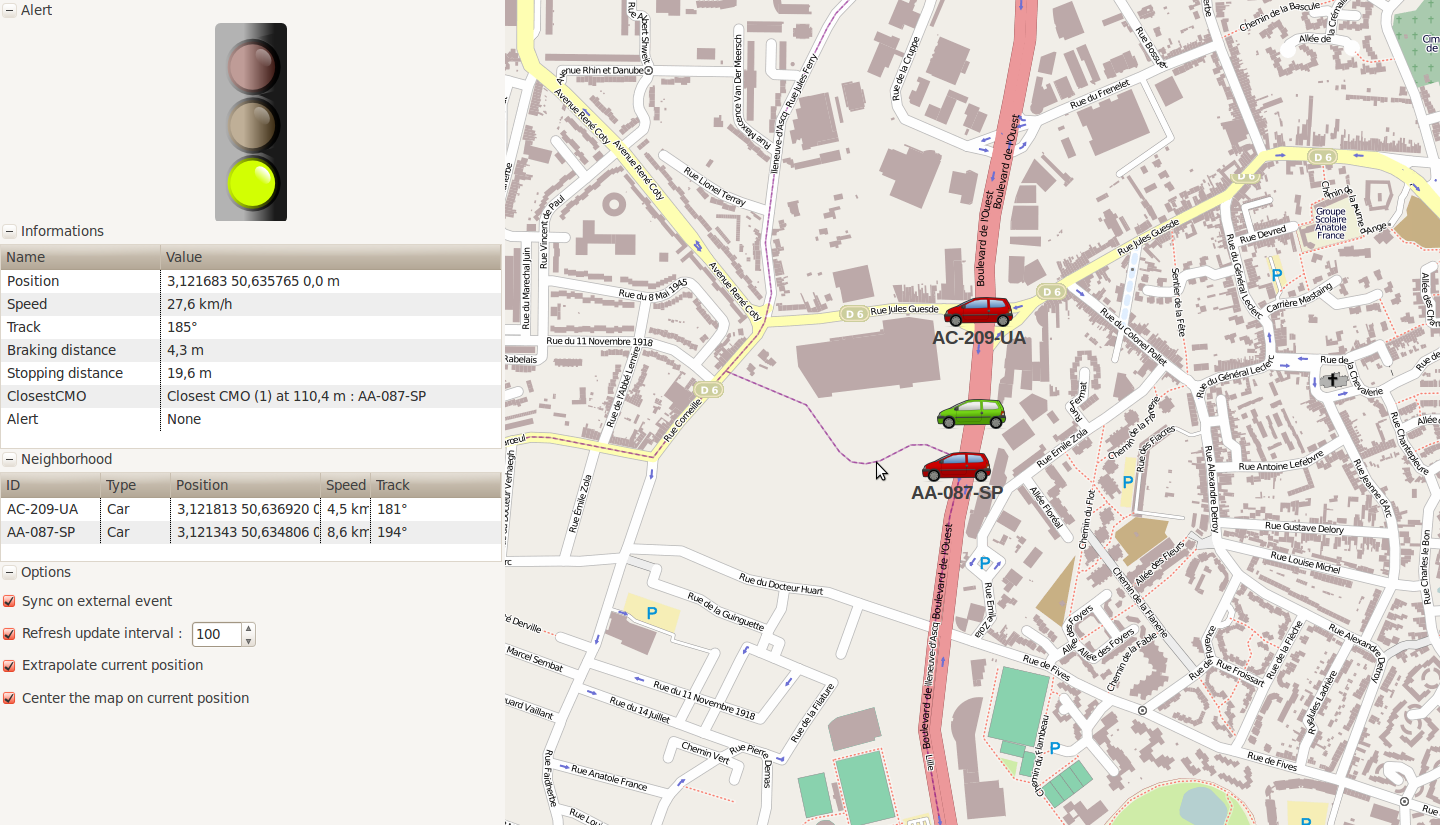
\includegraphics[width=1.01\textwidth]{Capture-GIS}
}

\frame{
	\frametitle{Geographic Information System (GIS) with weather}

  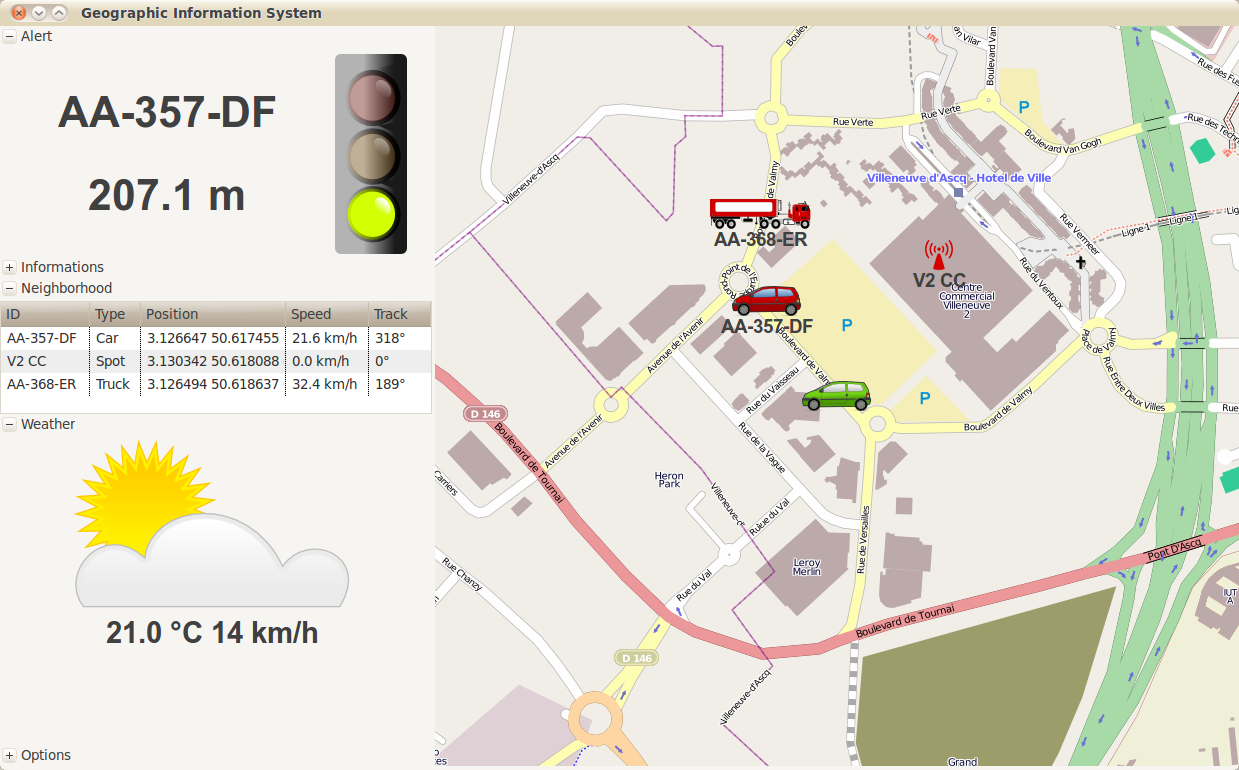
\includegraphics[width=1.01\textwidth]{Capture-GIS2}
}

\frame{
	\frametitle{Several type of CMO}

  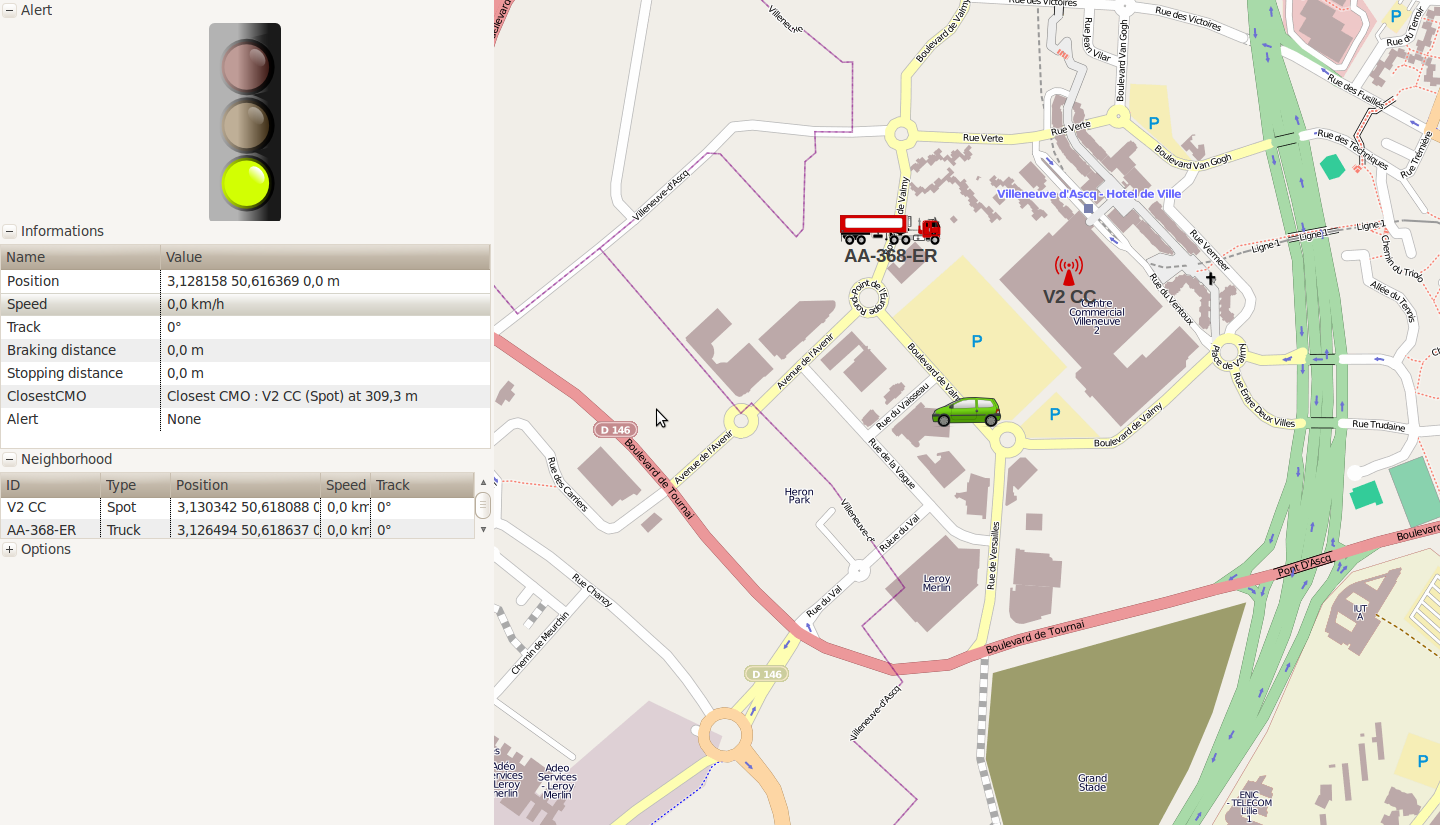
\includegraphics[width=1.01\textwidth]{Capture-GIS-type.png}
}



\frame{
	\frametitle{Software Architecture}

  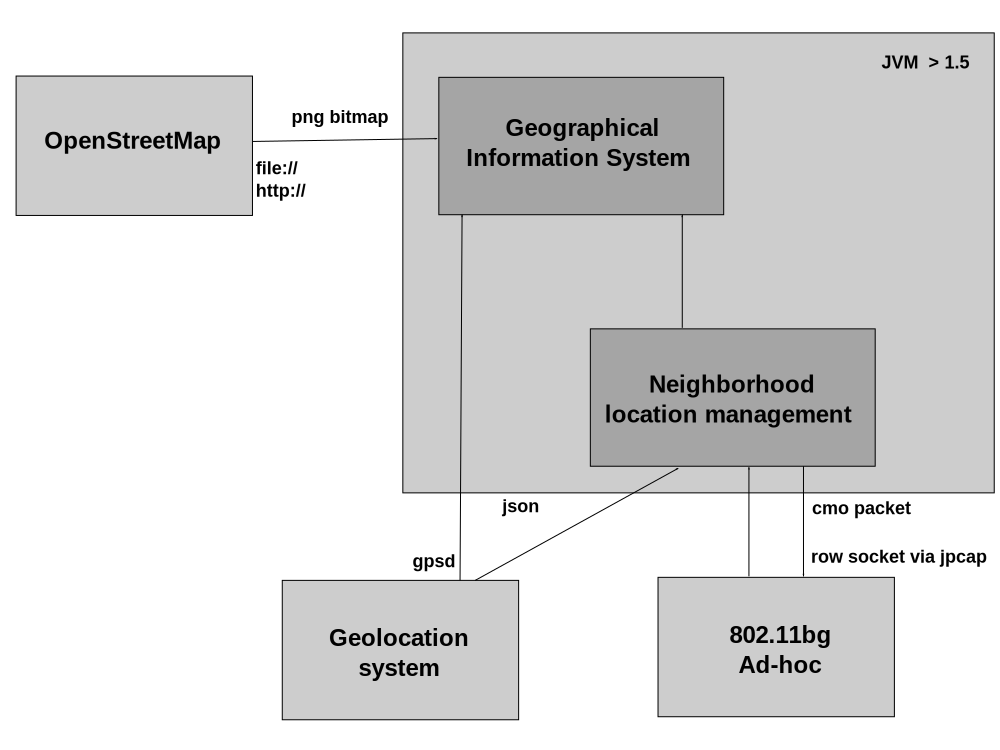
\includegraphics[width=0.8\textwidth]{architecture-cmo}
}


\frame{
	\frametitle{CMO Packet in payload of ethernet trame (type 0x0870)}

  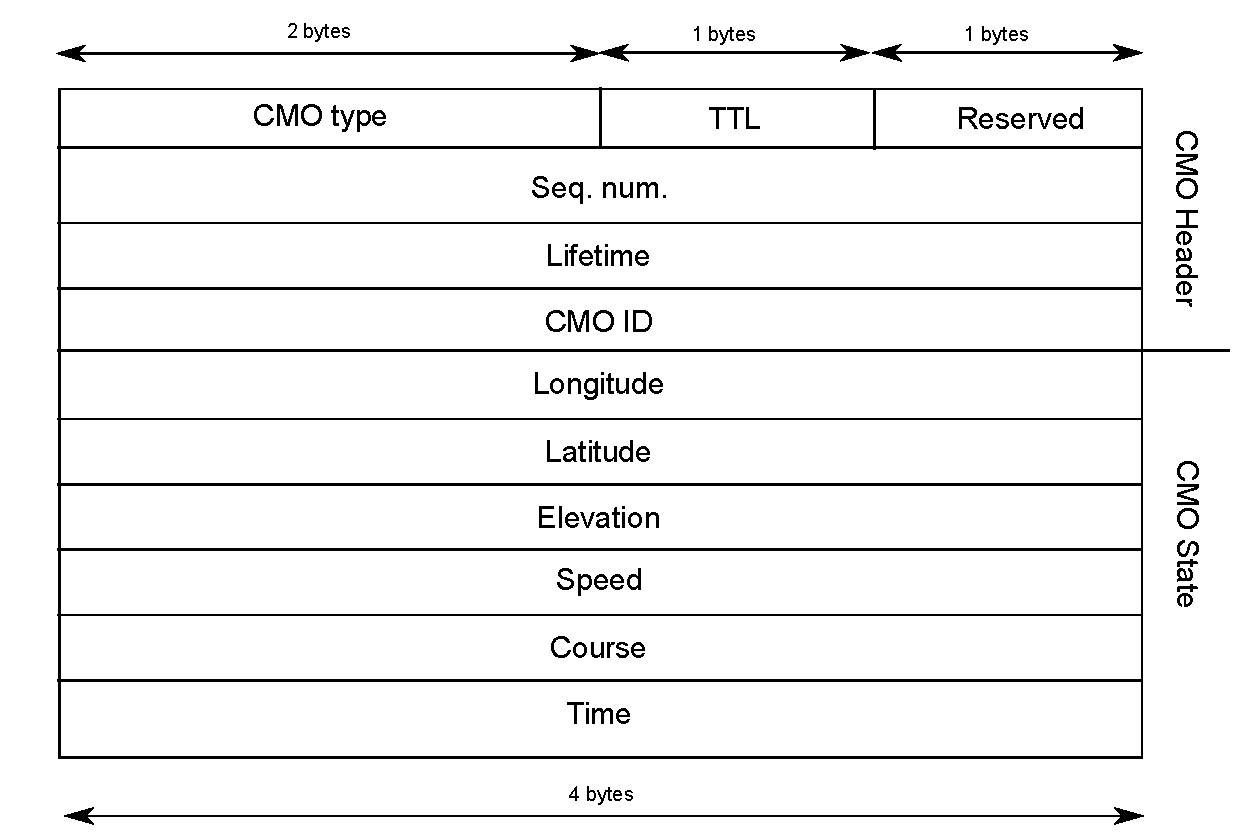
\includegraphics[width=0.9\textwidth]{packet-cmo}
}



\end{document}
